\documentclass[a4paper,12pt]{article}
% math font
\RequirePackage{amsmath}
\RequirePackage{amssymb}
\RequirePackage{amsthm}
\RequirePackage{mathtools}
\RequirePackage{newpxmath}
\usepackage{beton,euler}
\usepackage{tikz}
\usepackage{physics}
\usepackage[version=4]{mhchem}
\usepackage{chemfig}
\usepackage{pgfplots}
\usetikzlibrary{patterns,fillbetween}
\RequirePackage{geometry}
\geometry{%
	left=1cm,%
	right=1cm,%
	top=1.5cm,%
	bottom=1.5cm,%
	bindingoffset=0.8cm}
\begin{document}
	\centering
	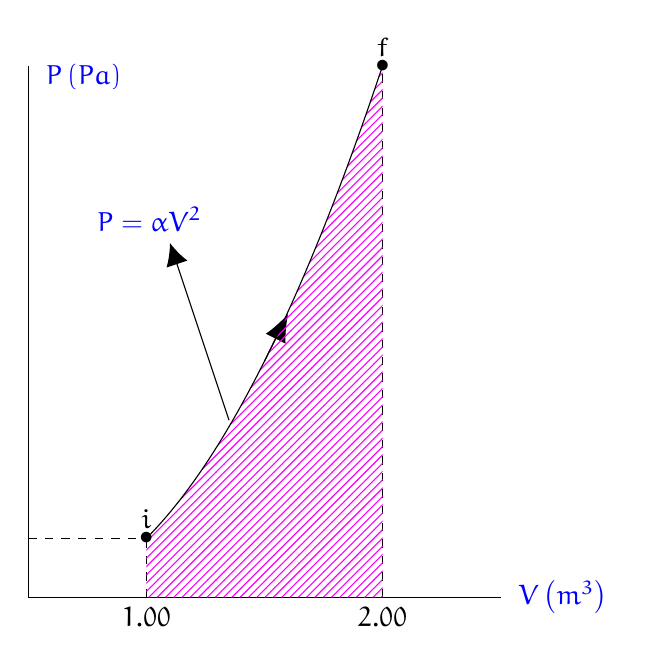
\begin{tikzpicture}[scale=1.5]
	\begin{scope}
	\coordinate [label=above:$i$] (i) at (1,0.5);
	\coordinate [label=above:$f$] (f) at (3,4.5);
	\draw (0,0)-- (4,0);
	\draw [dashed] (0,0.5)-- (1,0.5);
	\draw [dashed] (1,0)--(1,0.5);
	\draw [dashed] (3,0)--(3,4.5);
	\draw (0,0)-- (0,4.5);
	\draw(0,4.4) node [color=blue, right=.1cm]{$P\left(Pa\right)$};
	\draw(4,0) node [color=blue, right=.1cm]{$V\left(m^{3}\right)$};
	\draw [arrows = {-Latex[width=8pt, length=10pt]}] (2,2) -- (2.2,2.4);
	\draw [arrows = {-Latex[width=8pt, length=8pt]}] (1.7,1.5) -- (1.2,3);
	\path[domain=1:3,name path=C]plot(\x,{0.5*\x*\x});
	\path[domain=1:3,name path=X](1,0)node[below]{$ 1.00 $}--(3,0)node[below]{$ 2.00 $};
	%\tikzfillbetween[of={C and X}]{pattern=bricks,pattern color=magenta};
	\tikzfillbetween[of={C and X}]{pattern=north east lines,pattern color=magenta};
	\draw[domain=1:3,samples=50,black]plot(\x,{0.5*\x*\x});
	\node[right,text=blue] at (0.5,3.2){$ \displaystyle P=\alpha V^{2}$};
	\draw (1,0.5) node {$\bullet$};
	\draw (3,4.5) node {$\bullet$};
	\end{scope}
	\end{tikzpicture}
\end{document}